% Auswertung Emissionssektrum:
% Grenzwinkel: 5,6°
% min. Wellenänge: 39,31 pm
% max. Energie Bremsberg: 31,54 keV
% Auswertung Detailspektrum
% K_beta Linie Halbwertsbreite: 0,4°
% K_beta Linie min: 20,10° mit Energie 8956,705134376347eV
% K_beta Linie max: 20,50° mit Energie 8789,245217800455eV
% K_beta Linie max: 20,20° mit Energie 8914,203896517447eV
% K_beta Auflösungsvermögen A: 53,23186634025094
% ----------------
% K_alpha Linie Halbwertsbreite: 0,45°
% K_alpha Linie min: 22,30° mit Energie 8111,763305657744eV
% K_alpha Linie max: 22,75° mit Energie 7959,584434702297eV
% K_alpha Linie max: 22,60° mit Energie 8009,617524536037eV
% K_alpha Auflösungsvermögen A: 52,63291463688781
% ----------------
% sigma_1 exp: 3,5713015465602105
% sigma_2 exp: 12,22058064763327
% sigma_3 exp: 22,0875728042239
% ----------------
% sigma_1 theo: 3,5713015465602105
% sigma_2 theo: 12,138311271922081
% sigma_3 theo: 24,039726162119393
% ----------------
% Theta_K_Sr_exp: 10,99°
% Theta_K_Zr_exp: 9,91°
% Theta_K_Br_exp: 13,13°
% Theta_K_Zn_exp: 19,84°
% Theta_K_Ga_exp: 17,21°
% ----------------
% E_Sr exp: 16146,119558680297 eV
% E_Zr exp: 17885,183610259875 eV
% E_Br exp: 13550,104011791671 eV
% E_Zn exp: 9069,259432194094 eV
% E_Ga exp: 10403,247695213902 eV
% ----------------
% sigma_Sr exp: 4,326405561581936
% sigma_Zr exp: 4,606220593256381
% sigma_Br exp: 4,098435453201631
% sigma_Zn exp: 4,6679672621877195
% sigma_Ga exp: 3,8674501840169953
% ----------------
% a_sqrt: 3,828+/-0,009
% Rydberg exp(a): 14,65+/-0,07 eV
% b_sqrt: -1,81+/-0,28
% b: 3,3+/-1,0
\section{Auswertung}
\label{sec:Auswertung}
\subsection{Überprüfung der Bragg Bedingung}
In Abbildung \ref{fig:Bragg} sind die Messdaten zur Überprüfung der
Bragg-Bedingung der Röntgenstahlen auf ein LiF-Gitter dargestellt.
Anhand dieser Abbildung wird das Maximum bei $\theta_{\text{exp.}} = 14\,\unit{\degree}$
abgelesen. Der theoretische Braggwinkel lautet $\theta_{\text{theo.}} = 14\,\unit{\degree}$.
\begin{figure}[H]
  \centering
  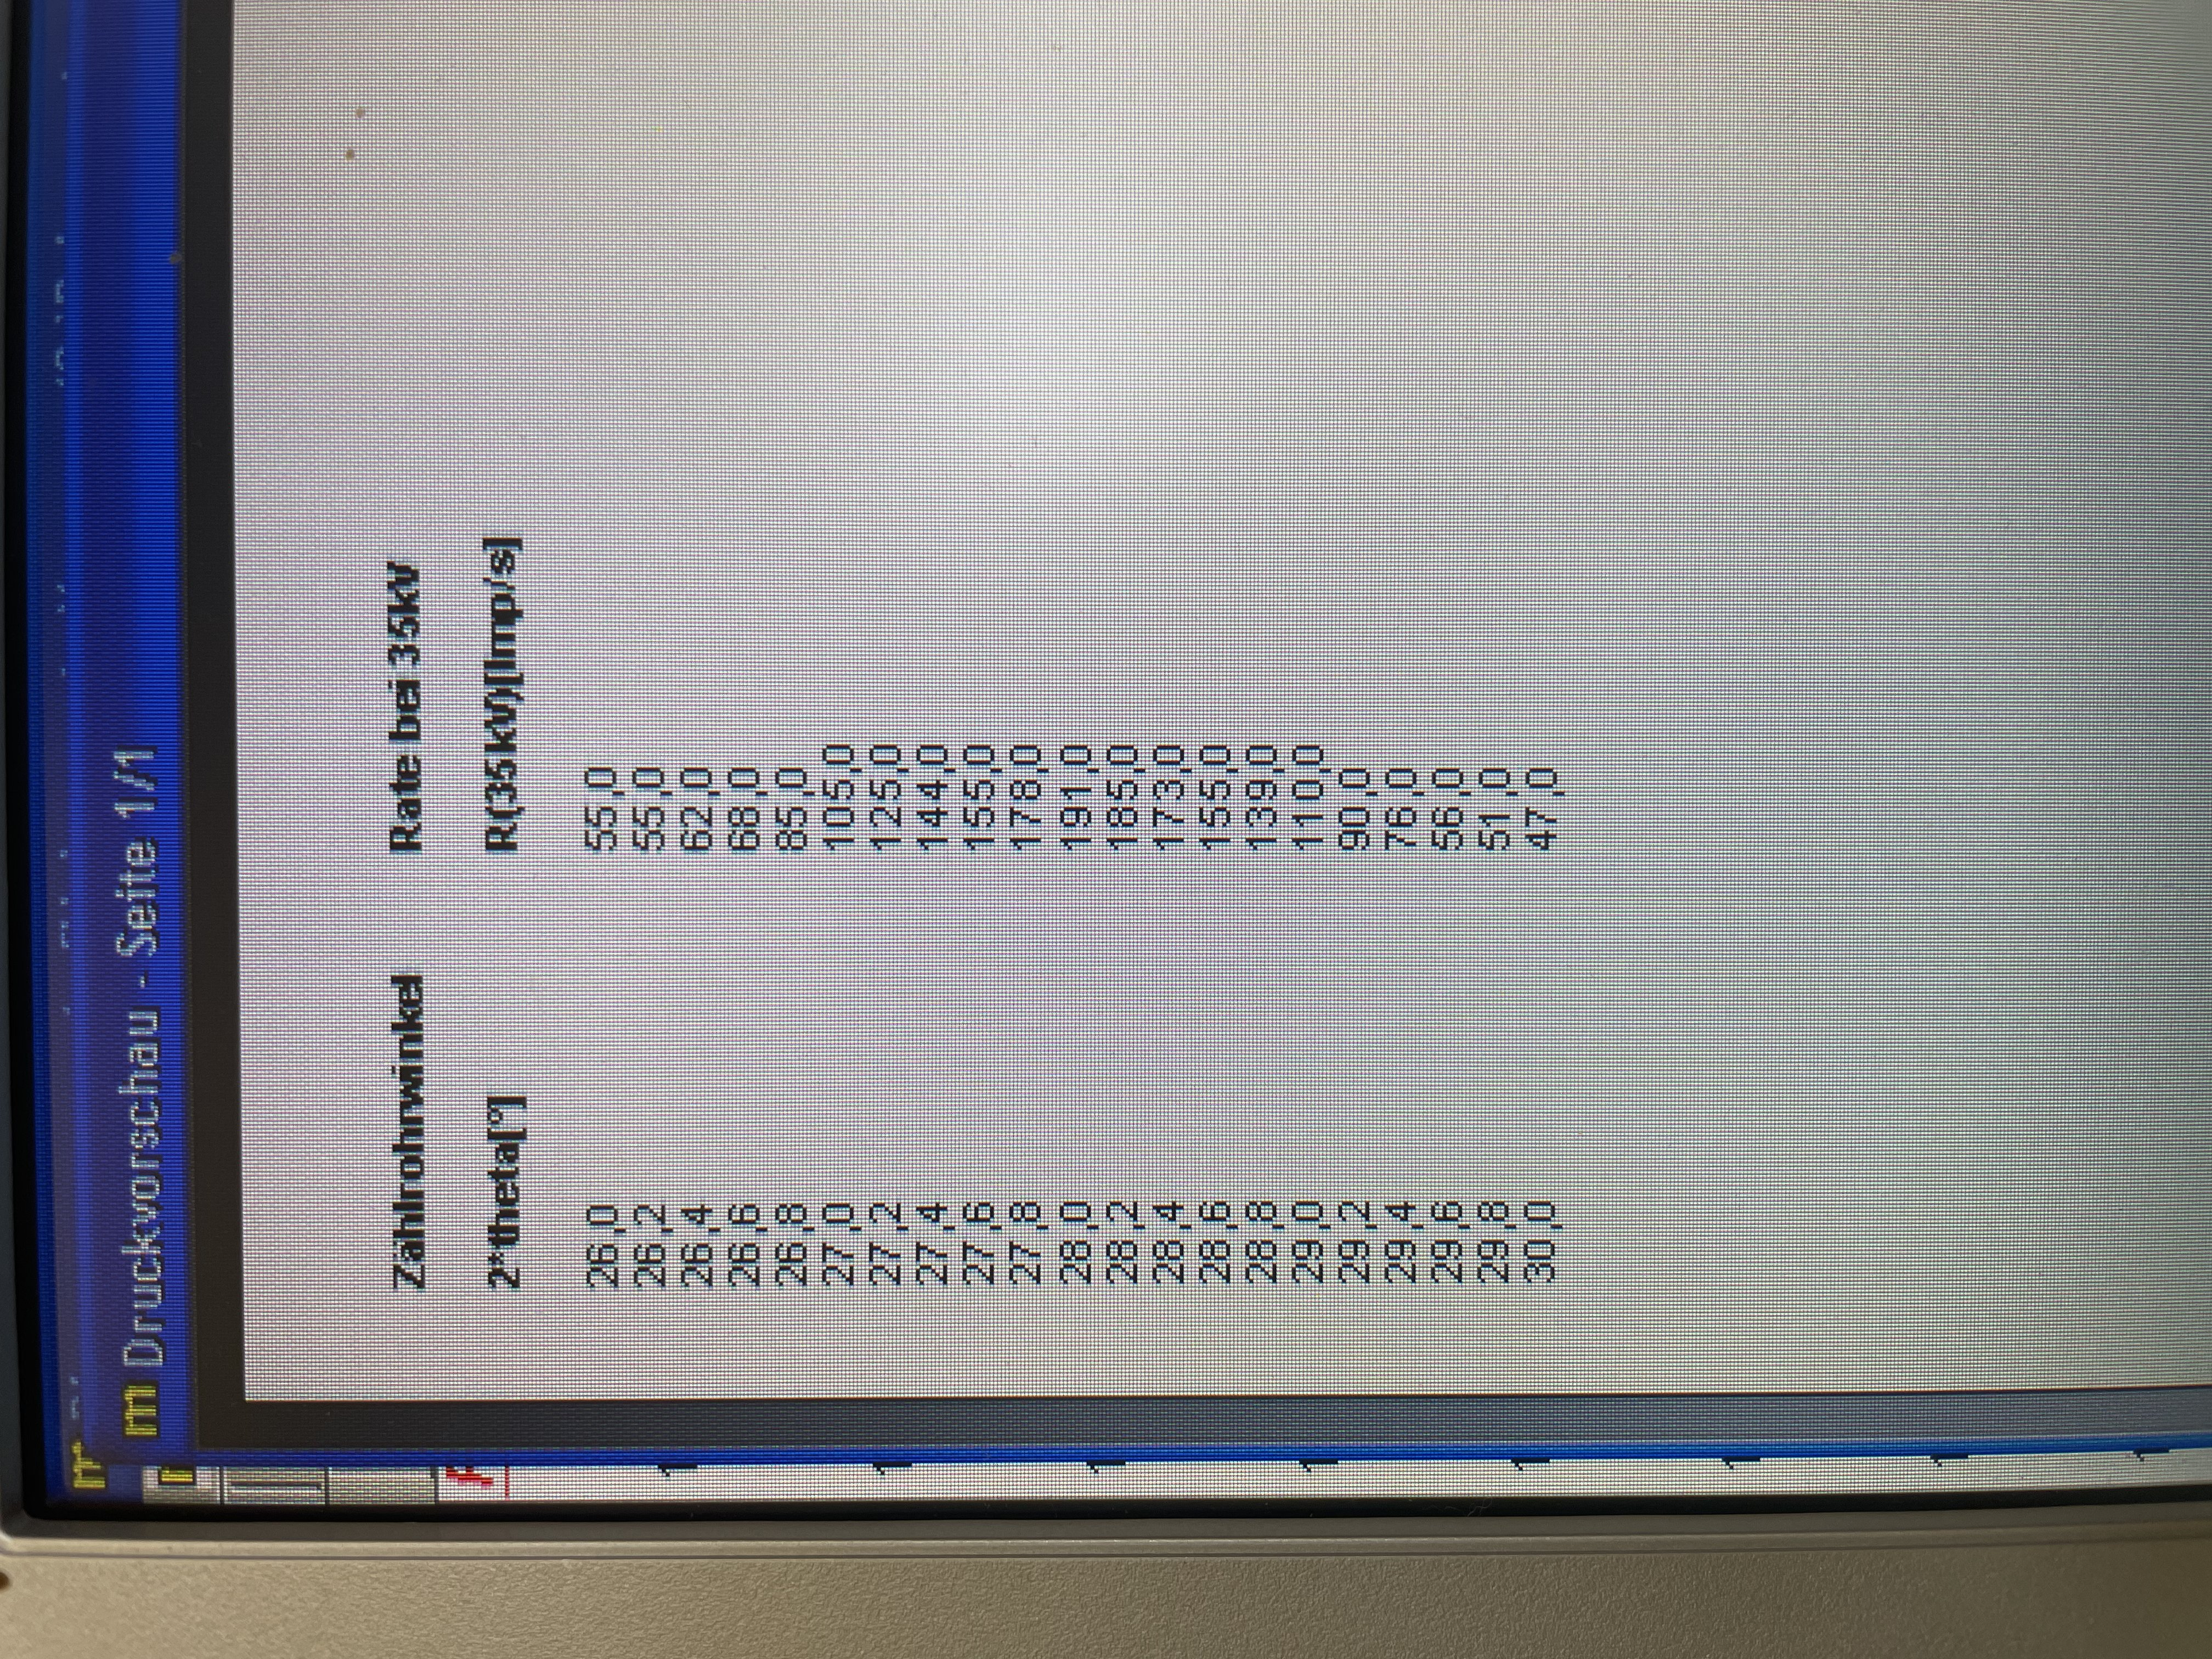
\includegraphics{content/Plots/Bragg.pdf}
  \caption{Messdaten zur Überprüfung der Bragg-Bedinung.}
  \label{fig:Bragg}
\end{figure}

\subsection{Emissionsspektrum einer Cu-Röntgenröhre}
Die Messdaten des Emissionsspektrums einer Cu-Röntgenröhre sind in der 
Abbildung \ref{fig:Emissionsspektrum} abgebildet. Zusätzlich sind in dieser
Abbildung der Bremsberg, die $K_{\alpha}$- und $K_{\beta}$-Linien markiert.
Aus der Graphik lassen sich 
\begin{align*}
  K_{\alpha} &= 22,6\,\unit{\degree} \\
  K_{\alpha} &= 20,2\,\unit{\degree}
\end{align*}
bestimmen. Der abgelesene Grenzwinkel $\theta_{\text{Grenz}}$ lautet etwa
$$\theta_{\text{Grenz}} = 5,6\,\unit{\degree}\,.$$ Damit lässt sich durch Umstellen der Gleichung
\ref{eqn:Bragg_Bedingung} die minimale Wellenlänge und mit der Gleichung \ref{eqn:} die maximale Energie des Bremsbergs
berechnen. Daraus folgt
\begin{align*}
  \lambda_{\text{min}} &= 39,31\,\unit{\pico\metre}\\
  E_{\text{max}} &= 31,54\,\unit{\kilo\eV}\,.
\end{align*}

\begin{figure}[H]
  \centering
  \includegraphics{content/Plots/Emissionsspektrum.pdf}
  \caption{Messdaten des Emissionsspektrum einer Cu-Röhre.}
  \label{fig:Emissionsspektrum}
\end{figure}
Um das Auflösungsvermögen der Apparatur zu bestimmen, wird der Ausschnitt der $K_{\alpha}$-
und $K_{\beta}$-Linien in der Abbildung \ref{fig:Detailspektrum} dargestellt. Innerhalb dieser Abbildung
sind die Halbwertsbreiten der $K_{\alpha}$ und $K_{\beta}$-Linien eingezeichnet. 
\begin{figure}[H]
  \centering
  \includegraphics{content/Plots/Detailspektrum.pdf}
  \caption{Detailspektrum der Cu-Röhre der $K_{\alpha}-$ und $K_{\beta}$-Linien.}
  \label{fig:Detailspektrum}
\end{figure}

\subsection{Absorptionsspektrum fünf verschiedener Materialien}
% \begin{figure}
%   \centering
%   \includegraphics{plot.pdf}
%   \caption{Plot.}
%   \label{fig:plot}
% \end{figure}
